% Latex-Formular für das Deckblatt des Physikpraktiums in Hannover
%%%%%%%%%%%%%%%%%%%%%%%%%%%%%%%%%%%%%%%%%%%%%%%%%%%%%%%%%%%%%%%%%%%%%%%%%%%%%%%%
% Diese Datei steht unter der Lizenz CC-BY-SA 4.0 . Sie darf kopiert, verändert
% und weitergegeben werden. Dabei müssen die Urheber genannt werden und die
% Lizenz beibehalten bleiben. Zu den Details siehe
% https://creativecommons.org/licenses/by-sa/4.0/
%%%%%%%%%%%%%%%%%%%%%%%%%%%%%%%%%%%%%%%%%%%%%%%%%%%%%%%%%%%%%%%%%%%%%%%%%%%%%%%%
% Autoren: Kim Weber, Kai-Martin Knaak, beide Leibniz-Universität Hannover
%%%%%%%%%%%%%%%%%%%%%%%%%%%%%%%%%%%%%%%%%%%%%%%%%%%%%%%%%%%%%%%%%%%%%%%%%%%%%%%%

\thispagestyle{empty}

\afterpage{%
\newgeometry{left=10mm,right=10mm,top=5mm,bottom=5mm}

\begin{Form}
	{\raisebox{-0.35\height}{
\includegraphics[width=0.4\textwidth]{Images/ap-logo_bw.pdf}}
	\hfill \Large Bericht zum Versuch: \underline{\TextField[name=Versuchsnummer,width=0.25 \textwidth,height=18pt,charsize=14pt,align=1]{}}}

\begin{tcolorbox}[coltitle=black,colbacktitle=black!10!white
		,title={Angaben zum Experiment}
		,sidebyside, sidebyside gap=1mm, righthand width=6cm, lower separated=false
		,toptitle=1mm
		,width=\linewidth-3mm]
	\begin{tabular}{lc}
		Name: & \underline{\TextField[name=Name, width=0.5 \textwidth,height=15pt,charsize=12pt]{}}\\
		Gruppennummer: & \underline{\TextField[name=GPNR, width=0.5 \textwidth,height=15pt,charsize=12pt]{}}\\
		Versuchsleiter:&\underline{\TextField[name=VSL,width=0.5 \textwidth,height=15pt,charsize=12pt]{}}\\
		Datum des Versuchs: & \underline{\TextField[name=VD,width=0.5 \linewidth,height=15pt,charsize=12pt]{}} \\
		Datum der Abgabe: & \underline{\TextField[name=VA,width=0.5 \textwidth,height=15pt,charsize=12pt]{}} \\
	\end{tabular}
	\tcblower
	\TextField[name=PT,width=1.0 \textwidth,height=80pt,charsize=64pt,align=1]{}
	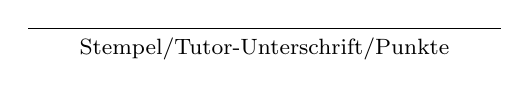
\begin{tikzpicture}
	\draw (0,0) -- node[below]{\footnotesize Stempel/Tutor-Unterschrift/Punkte}++(6,0);
	\end{tikzpicture}
\end{tcolorbox}

\begin{tcolorbox}[coltitle=black, colbacktitle=black!10!white
		,title={Allgemeines \hfill \janein }
		,toptitle=1mm
		,width=\linewidth-3mm]
	\begin{itemize}
		\setlength\itemsep{0em}
		\item{Abgabe des Berichts erfolgte pünktlich \kaestchen}
		\item{Äußere Form des Berichts ist angemessen \kaestchen}
		\item{Messdaten liegen dem Bericht bei \kaestchen}
		\item{Jede gedruckte Seite enthält Namen und Gruppennummer \kaestchen}
		\item{Es war keine Nachbesserung erforderlich \kaestchen}
	\end{itemize}
\end{tcolorbox}

\begin{tcolorbox}[coltitle=black, colbacktitle=black!10!white
		,title={Strukturierung und Dokumentation \hfill \janein }
		,toptitle=1mm
		,width=\linewidth-3mm]
	\begin{itemize}
		\setlength\itemsep{0em}
		\item{Der Bericht ist für sich stehend verständlich \hfill \kaestchen}
		\item{Rechenwege zur Ermittlung des Ergebnisses sind nachvollziehbar\hfill \kaestchen}
		\item{Unsicherheiten wurden richtig ermittelt (Fehlerfortpflanzung)\hfill \kaestchen}
		\item{Alle quantitativen Ergebnisse enthalten Angaben zur Messunsicherheit\hfill \kaestchen}
		\item{Messunsicherheiten und Ergebnisse werden diskutiert\hfill \kaestchen}
	\end{itemize}

\end{tcolorbox}
	\begin{tcolorbox}[coltitle=black, colbacktitle=black!10!white
		,title={Graphische Darstellung \hfill \janein }
		,toptitle=1mm
		,width=\linewidth-3mm]
	\begin{itemize}
		\setlength\itemsep{0em}
		\item{Bildunterschriften sind aussagekräftig \hfill \kaestchen}
		\item{Achsen sind vollständig bezeichnet und sinnvoll skaliert \hfill \kaestchen}
		\item{Messunsicherheiten sind mit Fehlerbalken dargestellt \hfill \kaestchen}
		\item{Bei Fit-Analysen sind alle relevanten Parameter angegeben \hfill \kaestchen}
		\item{Bei übernommenen Bildern ist die Quelle angegeben \hfill \kaestchen}
	\end{itemize}
\end{tcolorbox}

\begin{tcolorbox}[coltitle=black, colbacktitle=black!10!white
		,title={Anmerkungen}
		,sidebyside, sidebyside gap=1mm
		,toptitle=1mm
		,lower separated=false
		,width=\linewidth-3mm]
	\TextField[name=FB,multiline,width=\textwidth,height=48mm]{}%
	\tcblower
	\TextField[name=FB,multiline,width=\textwidth,height=48mm]{}%
\end{tcolorbox}

\scriptsize Deckblatt Physikpraktikum, Version 3.1 / \today
\hfill Kim Weber, Kai-Martin Knaak, Lizenz: {\href{https://creativecommons.org/licenses/by-sa/4.0/}{CC BY-SA 4.0}}

\end{Form}

\restoregeometry
}

